%% ----------------------------------------------------------------
%% Introduction.tex
%% 364
%% ---------------------------------------------------------------- 
\chapter{Introduction} \label{Chapter:Introduction}

%Introduction and Conclusion shouldn't include anything that it's not in the other parts.

%Only talk about the project itself at the introduction and NEVER AGAIN.

%Check that your paper is focused. Choose the point of the paper and its key conclusion before you begin writing, stick to your choices, and write the paper so that the reader gets the point already in the abstract and in the introduction. Leave  out results that are not required for supporting the key conclusion, or safely tuck them away in the supplementary information document. When editing, if you feel that your paper loses its focus at some point, take a step back and do a major rewrite.

%Check that there is a clear question and a clear answer—it is all too common to focus on your results and what you have done, instead of stating and then solving a problem. Your results are meaningful only if they solve a meaningful problem. Remember that your paper is neither an account of your work nor a lab diary; it should be a story of an important problem and its solution. Emphasise the problem, both in the Introduction where it should really stand out, and in the Results section and the Discussion. Make it clear to the reader how each result contributes to solving the problem, and what the implications of solving the problem are.

%\begin{enumerate}
%\item What am I going to prove?
%\item Why does this matter?
%\end{enumerate}
%% --------------------------------------------------------
%\begin{figure}[!htb]
%  \centering
 % \subfigure[The left caption]{
  %  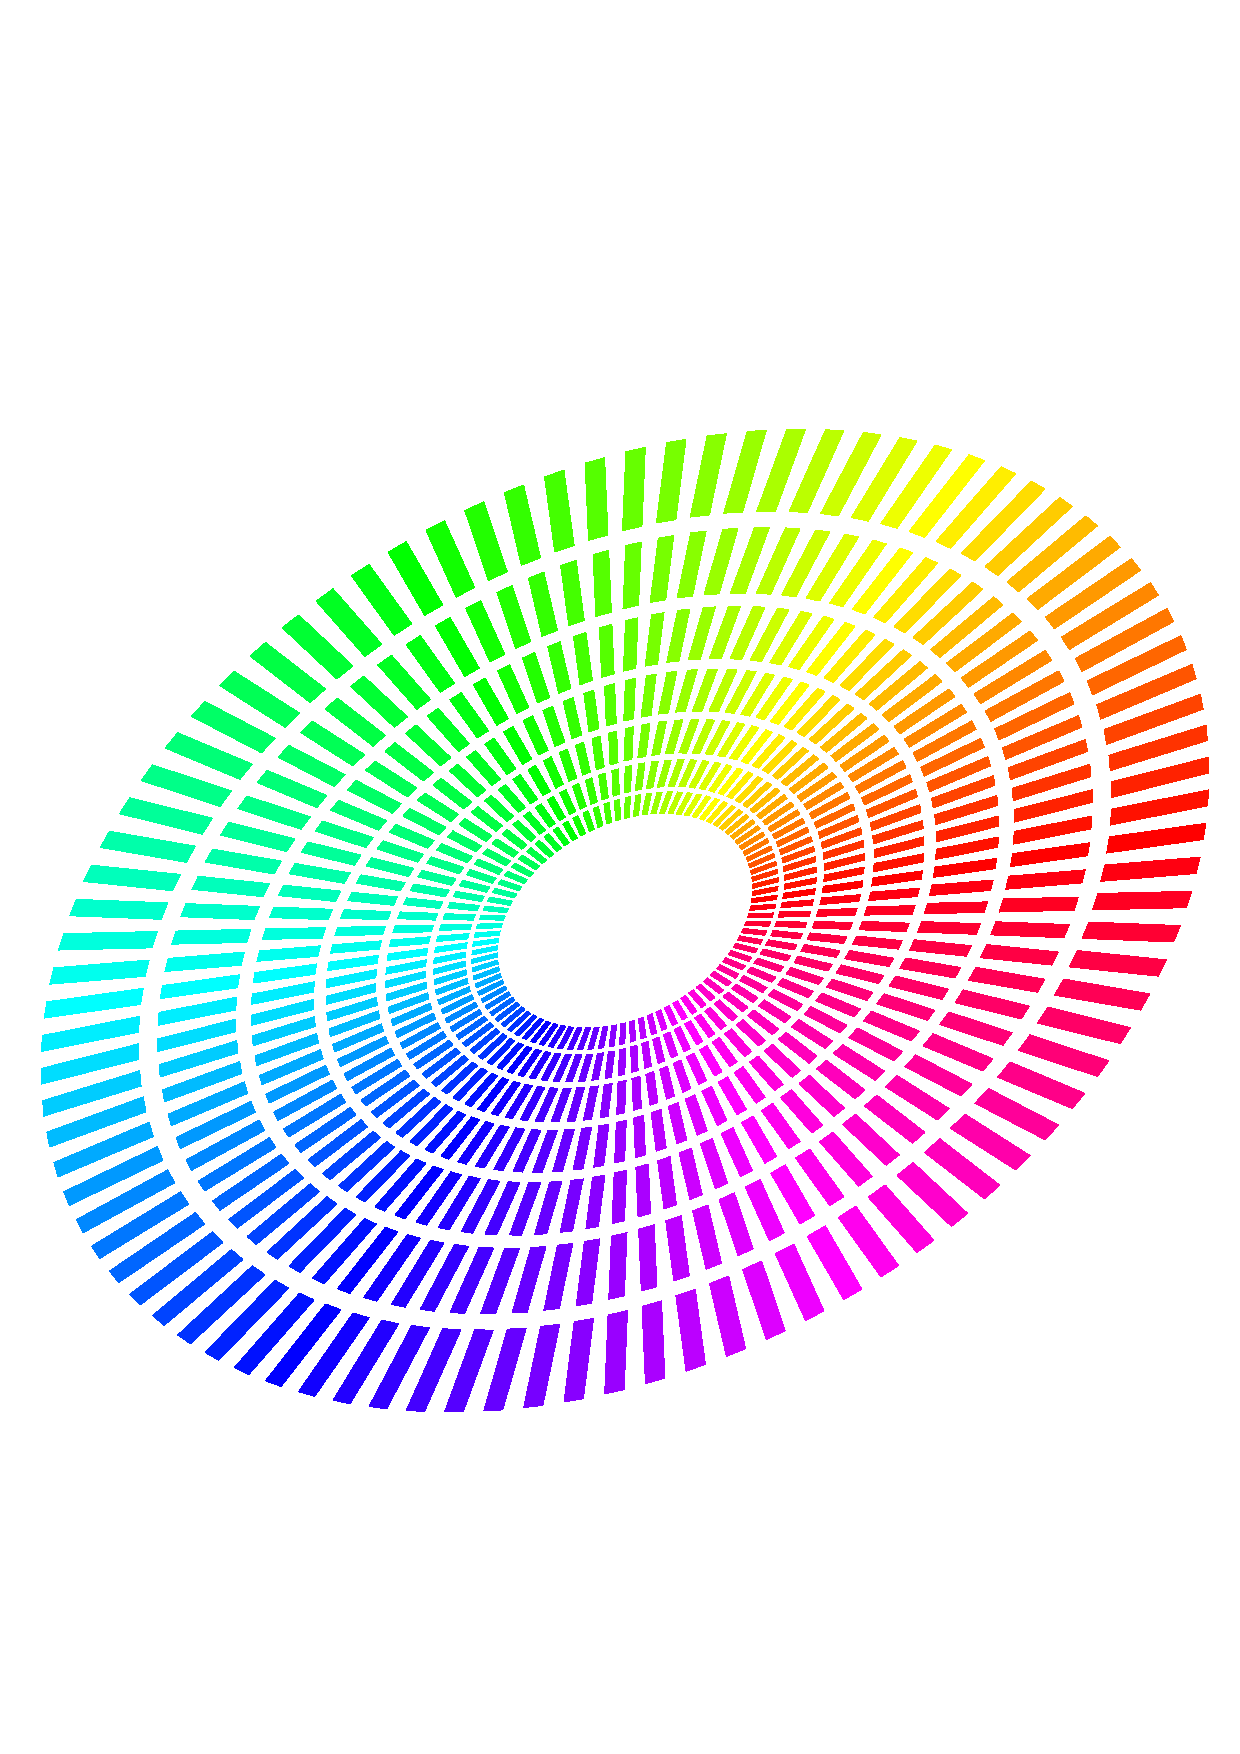
\includegraphics[width=4.2cm]{figure}
   % \label{Figure:figsubex:left}
  %}
  %\subfigure[The right caption]{
   % 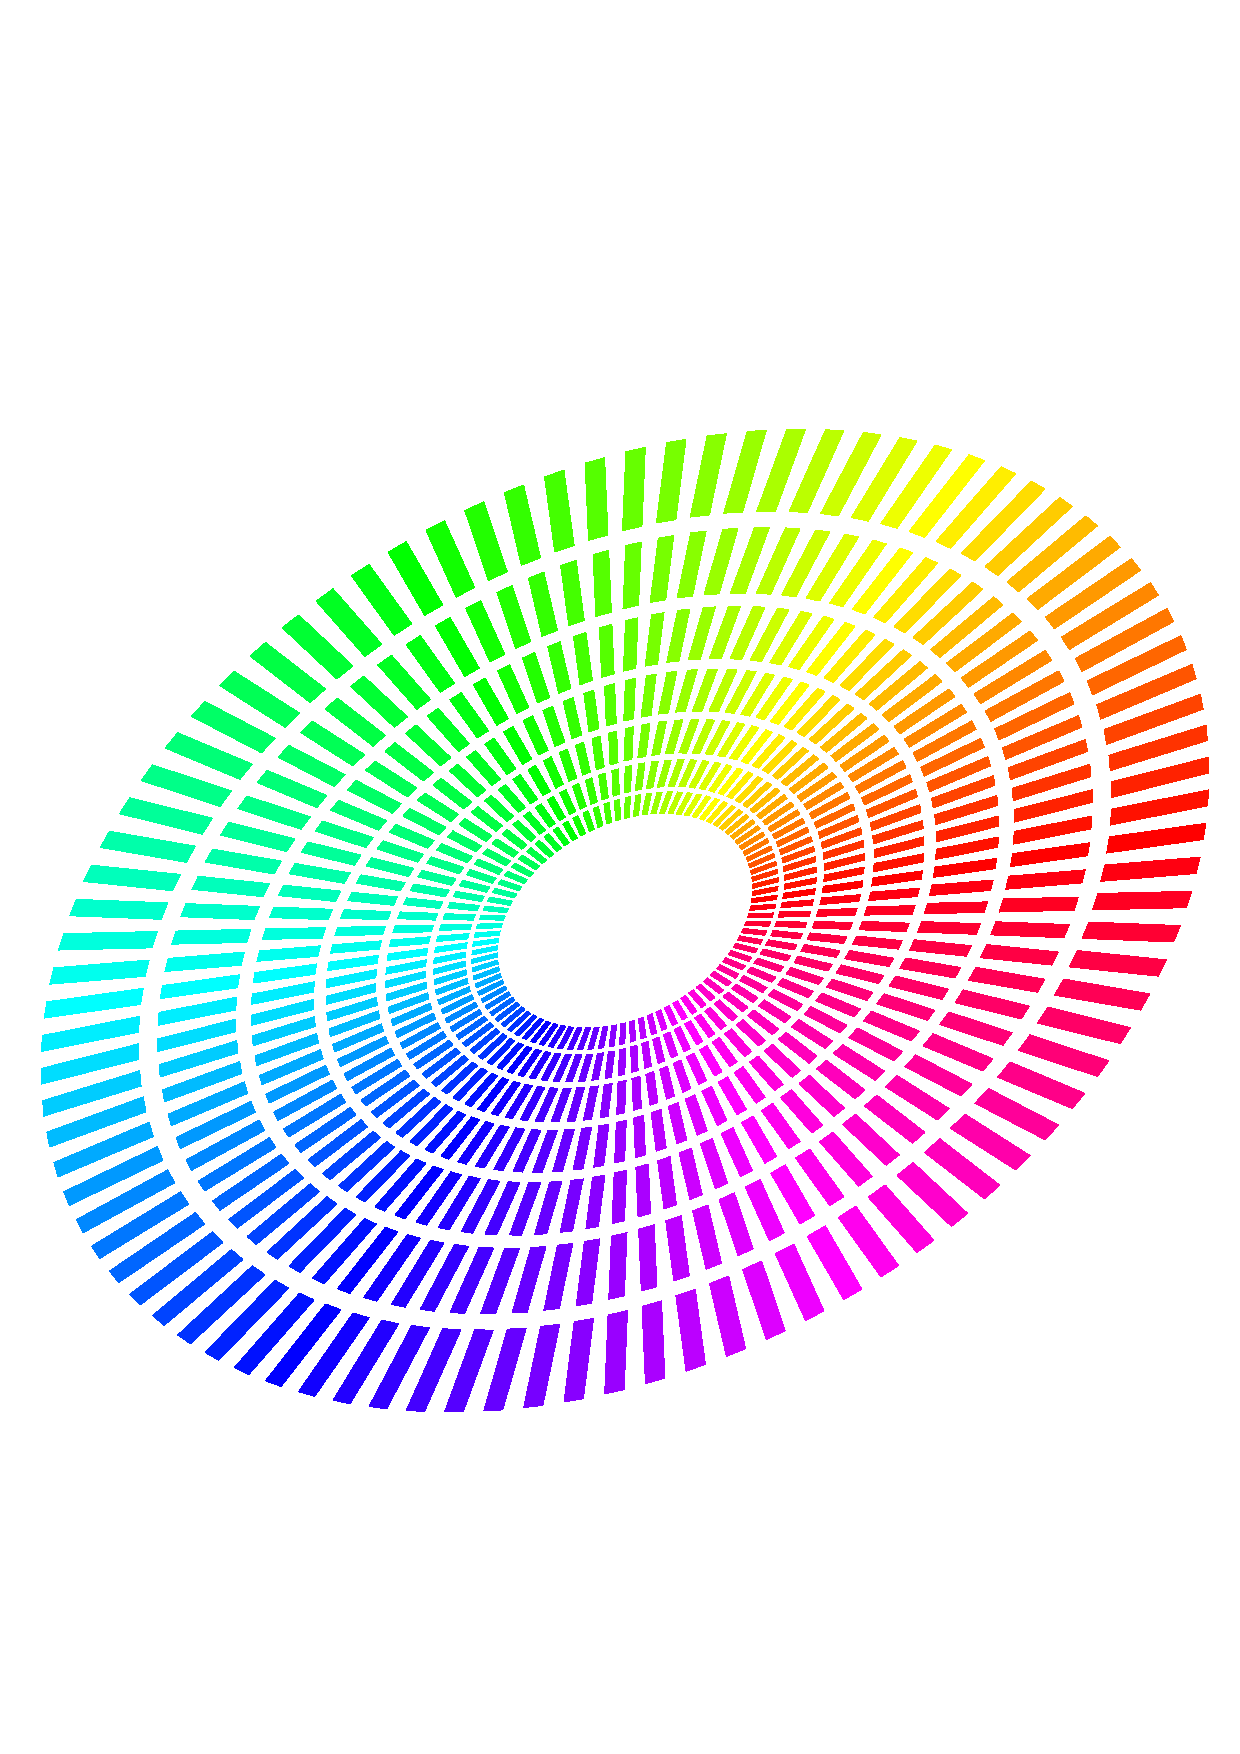
\includegraphics[width=4.2cm]{figure}
    %\label{Figure:figsubex:right}
  %}
  %\caption{A doubly colourful picture.}
  %\label{Figure:figsubex}
%\end{figure}

Although the recent arrival of deep learning has introduced unprecedented improvements in many fields, it also brings techniques that are remarkably difficult to understand. Many layers of neurons stack on each other and build complex networks of interactions, with the information distributed and therefore meaningless if we look at an isolated unit. The outcome emerges from the interaction of them all, and this indivisibility is what makes them so hard to grasp. Without being able to look inside, debugging efforts are futile, and we lose the benefits of learning from the acquired representations.

Biomedical research is one of the fields in which deep learning has overcome previous techniques, due to the complex interactions that occur in the networks been studied there, from gene regulatory networks in the molecular level to macro-ecosystems. One of the domains where it excels can be found in the sequential data at the cellular level: DNA, RNA and protein chains. However, the lack of interpretability is again a significant issue since we do not fully understand the underlying processes being modelled and uncritically accepting an outcome is not the best option. If experts in the field can somehow verify what the system is doing, they will be able to contrast it with their knowledge to both spot spurious rules being learned and update their knowledge with new valuable pieces.

The field of image processing, which is one of the earliest to embrace deep learning, has started to work already in the development of interpretability techniques that may cope with these issues. They focus on capturing the intermediate representations that are formed in the hidden layers to understand what kind of features are learned at different layers (\textit{feature visualization}), as well as exploring which sections of the inputs contain the most crucial information for the system to make a decision (\textit{saliency maps}). Although there have been a few attempts to bring them to biological sequence problems, there is still much room for improvement. This project aims to explore ways to implement saliency map techniques into biological sequence problems; or more specifically, into protein secondary structure prediction, as one of the canonical sequence-to-sequence prediction problems in cellular biology.